
\begin{frame}[fragile]{Computable functions are continuous}

\begin{center}

    \begin{tikzpicture}[scale=1.25]
    \draw[red,thick] (0,3) parabola bend (0,3) (2,2.0);
    \draw[red,thick] (2,1.0) parabola bend (2,1.0) (4, 3.0); 
    \draw[red, fill=white] (2,2.0) circle (.1cm); 
    \draw[fill=blue] (2,1.0) circle (.1cm); 
    %\draw[loosely dotted] (0,0) grid (4,4);
    %\path[use as bounding box] (-2,-1) rectangle (5,5);
    \draw[->] (-0.2,0) -- (4.25,0) node[right] {$x$};
    \draw[->] (0,-0.25) -- (0,4.25) node[above] {$y$};
    \foreach \x/\xtext in {1/1, 2/2, 3/3}
    \draw[shift={(\x,0)}] (0pt,2pt) -- (0pt,-2pt) node[below] {};
    \foreach \y/\ytext in {1/1, 2/2, 3/3, 4/4}
    \draw[shift={(0,\y)}] (2pt,0pt) -- (-2pt,0pt) node[left] {};
   % \draw[dotted,line width=2pt] (0,1) -- (2,1);
    %\draw[dotted,line width=2pt] (2,1) -- (2,0);
    %\draw[dotted,line width=2pt] (0,2.21) -- (1.8,2.21);
    \%draw[dotted,line width=2pt] (1.8,2.21) -- (1.8,0);
    %\draw[green,line width=3pt] (0,0.5) -- (0,2.5);
    %\draw[green,line width=3pt] (4pt,0.5) -- (-4pt,0.5);
    %\draw[green,line width=3pt] (4pt,2.5) -- (-4pt,2.5);
    %\draw[green,line width=3pt] (0,0.5) -- (0,1.5);
    %\draw[green,line width=3pt] (4pt,0.5) -- (-4pt,0.5);
    %\draw[green,line width=3pt] (4pt,1.5) -- (-4pt,1.5);

%    \draw[blue,line width=3pt] (0.5,0) -- (3.5,0);
%   \draw[blue,line width=3pt] (0.5,4pt) -- (0.5,-4pt);
 %   \draw[blue,line width=3pt] (3.5,4pt) -- (3.5,-4pt);
 %     \draw[blue,line width=3pt] (1.0,0) -- (3.0,0);
   % \draw[blue,line width=3pt] (1.0,4pt) -- (1.0,-4pt);
   % \draw[blue,line width=3pt] (3.0,4pt) -- (3.0,-4pt);  
   %   \draw[blue,line width=3pt] (1.5,0) -- (2.5,0);
   % \draw[blue,line width=3pt] (1.5,4pt) -- (1.5,-4pt);
   % \draw[blue,line width=3pt] (2.5,4pt) -- (2.5,-4pt);  
%
    \end{tikzpicture}
\end{center}
\end{frame}

\addtocounter{framenumber}{-1}
\begin{frame}[fragile]{Computable functions are continuous}

\begin{center}

    \begin{tikzpicture}[scale=1.25]
    \draw[red,thick] (0,3) parabola bend (0,3) (2,2.0);
    \draw[red,thick] (2,1.0) parabola bend (2,1.0) (4, 3.0); 
    \draw[red, fill=white] (2,2.0) circle (.1cm); 
    \draw[fill=blue] (2,1.0) circle (.1cm); 
    %\draw[loosely dotted] (0,0) grid (4,4);
    %\path[use as bounding box] (-2,-1) rectangle (5,5);
    \draw[->] (-0.2,0) -- (4.25,0) node[right] {$x$};
    \draw[->] (0,-0.25) -- (0,4.25) node[above] {$y$};
    \foreach \x/\xtext in {1/1, 2/2, 3/3}
    \draw[shift={(\x,0)}] (0pt,2pt) -- (0pt,-2pt) node[below] {};
    \foreach \y/\ytext in {1/1, 2/2, 3/3, 4/4}
    \draw[shift={(0,\y)}] (2pt,0pt) -- (-2pt,0pt) node[left] {};
    \draw[dotted,line width=2pt] (0,1) -- (2,1);
    \draw[dotted,line width=2pt] (2,1) -- (2,0);
    %\draw[dotted,line width=2pt] (0,2.21) -- (1.8,2.21);
    \%draw[dotted,line width=2pt] (1.8,2.21) -- (1.8,0);
    %\draw[green,line width=3pt] (0,0.5) -- (0,2.5);
    %\draw[green,line width=3pt] (4pt,0.5) -- (-4pt,0.5);
    %\draw[green,line width=3pt] (4pt,2.5) -- (-4pt,2.5);
    %\draw[green,line width=3pt] (0,0.5) -- (0,1.5);
    %\draw[green,line width=3pt] (4pt,0.5) -- (-4pt,0.5);
    %\draw[green,line width=3pt] (4pt,1.5) -- (-4pt,1.5);

%    \draw[blue,line width=3pt] (0.5,0) -- (3.5,0);
%   \draw[blue,line width=3pt] (0.5,4pt) -- (0.5,-4pt);
 %   \draw[blue,line width=3pt] (3.5,4pt) -- (3.5,-4pt);
 %     \draw[blue,line width=3pt] (1.0,0) -- (3.0,0);
   % \draw[blue,line width=3pt] (1.0,4pt) -- (1.0,-4pt);
   % \draw[blue,line width=3pt] (3.0,4pt) -- (3.0,-4pt);  
   %   \draw[blue,line width=3pt] (1.5,0) -- (2.5,0);
   % \draw[blue,line width=3pt] (1.5,4pt) -- (1.5,-4pt);
   % \draw[blue,line width=3pt] (2.5,4pt) -- (2.5,-4pt);  
%
    \end{tikzpicture}
\end{center}
\end{frame}

\addtocounter{framenumber}{-1}
\begin{frame}[fragile]{Computable functions are continuous}

\begin{center}

    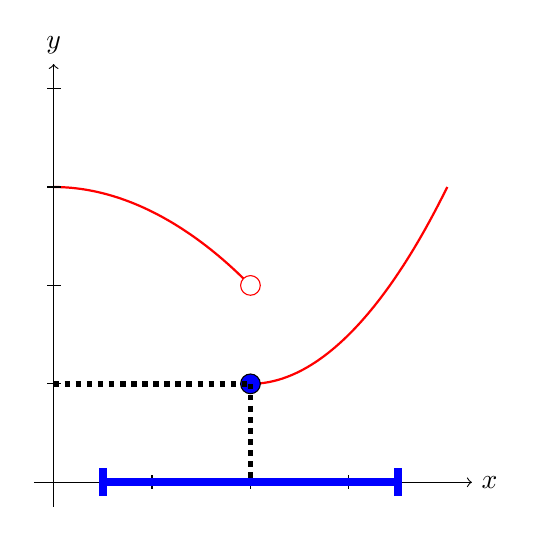
\begin{tikzpicture}[scale=1.25]
    \draw[red,thick] (0,3) parabola bend (0,3) (2,2.0);
    \draw[red,thick] (2,1.0) parabola bend (2,1.0) (4, 3.0); 
    \draw[red, fill=white] (2,2.0) circle (.1cm); 
    \draw[fill=blue] (2,1.0) circle (.1cm); 
    %\draw[loosely dotted] (0,0) grid (4,4);
    %\path[use as bounding box] (-2,-1) rectangle (5,5);
    \draw[->] (-0.2,0) -- (4.25,0) node[right] {$x$};
    \draw[->] (0,-0.25) -- (0,4.25) node[above] {$y$};
    \foreach \x/\xtext in {1/1, 2/2, 3/3}
    \draw[shift={(\x,0)}] (0pt,2pt) -- (0pt,-2pt) node[below] {};
    \foreach \y/\ytext in {1/1, 2/2, 3/3, 4/4}
    \draw[shift={(0,\y)}] (2pt,0pt) -- (-2pt,0pt) node[left] {};
    \draw[dotted,line width=2pt] (0,1) -- (2,1);
    \draw[dotted,line width=2pt] (2,1) -- (2,0);
    %\draw[dotted,line width=2pt] (0,2.21) -- (1.8,2.21);
    \%draw[dotted,line width=2pt] (1.8,2.21) -- (1.8,0);
    %\draw[green,line width=3pt] (0,0.5) -- (0,2.5);
    %\draw[green,line width=3pt] (4pt,0.5) -- (-4pt,0.5);
    %\draw[green,line width=3pt] (4pt,2.5) -- (-4pt,2.5);
    %\draw[green,line width=3pt] (0,0.5) -- (0,1.5);
    %\draw[green,line width=3pt] (4pt,0.5) -- (-4pt,0.5);
    %\draw[green,line width=3pt] (4pt,1.5) -- (-4pt,1.5);

    \draw[blue,line width=3pt] (0.5,0) -- (3.5,0);
   \draw[blue,line width=3pt] (0.5,4pt) -- (0.5,-4pt);
    \draw[blue,line width=3pt] (3.5,4pt) -- (3.5,-4pt);
 %     \draw[blue,line width=3pt] (1.0,0) -- (3.0,0);
   % \draw[blue,line width=3pt] (1.0,4pt) -- (1.0,-4pt);
   % \draw[blue,line width=3pt] (3.0,4pt) -- (3.0,-4pt);  
   %   \draw[blue,line width=3pt] (1.5,0) -- (2.5,0);
   % \draw[blue,line width=3pt] (1.5,4pt) -- (1.5,-4pt);
   % \draw[blue,line width=3pt] (2.5,4pt) -- (2.5,-4pt);  
%
    \end{tikzpicture}
\end{center}
\end{frame}


\addtocounter{framenumber}{-1}
\begin{frame}[fragile]{Computable functions are continuous}

\begin{center}

    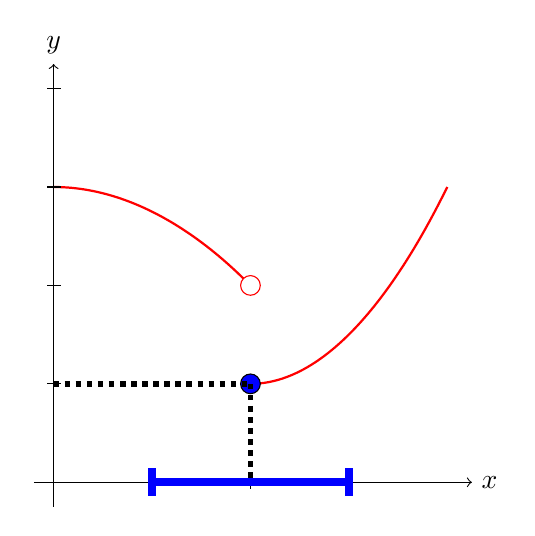
\begin{tikzpicture}[scale=1.25]
    \draw[red,thick] (0,3) parabola bend (0,3) (2,2.0);
    \draw[red,thick] (2,1.0) parabola bend (2,1.0) (4, 3.0); 
    \draw[red, fill=white] (2,2.0) circle (.1cm); 
    \draw[fill=blue] (2,1.0) circle (.1cm); 
    %\draw[loosely dotted] (0,0) grid (4,4);
    %\path[use as bounding box] (-2,-1) rectangle (5,5);
    \draw[->] (-0.2,0) -- (4.25,0) node[right] {$x$};
    \draw[->] (0,-0.25) -- (0,4.25) node[above] {$y$};
    \foreach \x/\xtext in {1/1, 2/2, 3/3}
    \draw[shift={(\x,0)}] (0pt,2pt) -- (0pt,-2pt) node[below] {};
    \foreach \y/\ytext in {1/1, 2/2, 3/3, 4/4}
    \draw[shift={(0,\y)}] (2pt,0pt) -- (-2pt,0pt) node[left] {};
    \draw[dotted,line width=2pt] (0,1) -- (2,1);
    \draw[dotted,line width=2pt] (2,1) -- (2,0);
    %\draw[dotted,line width=2pt] (0,2.21) -- (1.8,2.21);
    \%draw[dotted,line width=2pt] (1.8,2.21) -- (1.8,0);
    %\draw[green,line width=3pt] (0,0.5) -- (0,2.5);
    %\draw[green,line width=3pt] (4pt,0.5) -- (-4pt,0.5);
    %\draw[green,line width=3pt] (4pt,2.5) -- (-4pt,2.5);
    %\draw[green,line width=3pt] (0,0.5) -- (0,1.5);
    %\draw[green,line width=3pt] (4pt,0.5) -- (-4pt,0.5);
    %\draw[green,line width=3pt] (4pt,1.5) -- (-4pt,1.5);

%    \draw[blue,line width=3pt] (0.5,0) -- (3.5,0);
 %  \draw[blue,line width=3pt] (0.5,4pt) -- (0.5,-4pt);
  %  \draw[blue,line width=3pt] (3.5,4pt) -- (3.5,-4pt);
      \draw[blue,line width=3pt] (1.0,0) -- (3.0,0);
    \draw[blue,line width=3pt] (1.0,4pt) -- (1.0,-4pt);
    \draw[blue,line width=3pt] (3.0,4pt) -- (3.0,-4pt);  
   %   \draw[blue,line width=3pt] (1.5,0) -- (2.5,0);
   % \draw[blue,line width=3pt] (1.5,4pt) -- (1.5,-4pt);
   % \draw[blue,line width=3pt] (2.5,4pt) -- (2.5,-4pt);  
%
    \end{tikzpicture}
\end{center}
\end{frame}



\addtocounter{framenumber}{-1}
\begin{frame}[fragile]{Computable functions are continuous}

\begin{center}

    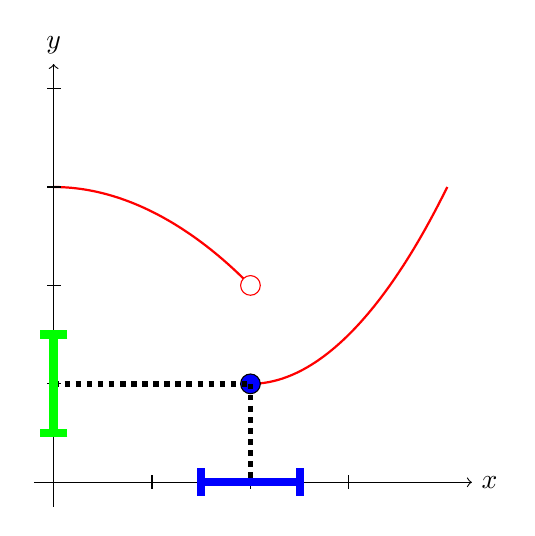
\begin{tikzpicture}[scale=1.25]
    \draw[red,thick] (0,3) parabola bend (0,3) (2,2.0);
    \draw[red,thick] (2,1.0) parabola bend (2,1.0) (4, 3.0); 
    \draw[red, fill=white] (2,2.0) circle (.1cm); 
    \draw[fill=blue] (2,1.0) circle (.1cm); 
    %\draw[loosely dotted] (0,0) grid (4,4);
    %\path[use as bounding box] (-2,-1) rectangle (5,5);
    \draw[->] (-0.2,0) -- (4.25,0) node[right] {$x$};
    \draw[->] (0,-0.25) -- (0,4.25) node[above] {$y$};
    \foreach \x/\xtext in {1/1, 2/2, 3/3}
    \draw[shift={(\x,0)}] (0pt,2pt) -- (0pt,-2pt) node[below] {};
    \foreach \y/\ytext in {1/1, 2/2, 3/3, 4/4}
    \draw[shift={(0,\y)}] (2pt,0pt) -- (-2pt,0pt) node[left] {};
    \draw[dotted,line width=2pt] (0,1) -- (2,1);
    \draw[dotted,line width=2pt] (2,1) -- (2,0);
    %\draw[dotted,line width=2pt] (0,2.21) -- (1.8,2.21);
    \%draw[dotted,line width=2pt] (1.8,2.21) -- (1.8,0);
    %\draw[green,line width=3pt] (0,0.5) -- (0,2.5);
    %\draw[green,line width=3pt] (4pt,0.5) -- (-4pt,0.5);
    %\draw[green,line width=3pt] (4pt,2.5) -- (-4pt,2.5);
    \draw[green,line width=3pt] (0,0.5) -- (0,1.5);
    \draw[green,line width=3pt] (4pt,0.5) -- (-4pt,0.5);
    \draw[green,line width=3pt] (4pt,1.5) -- (-4pt,1.5);

%    \draw[blue,line width=3pt] (0.5,0) -- (3.5,0);
 %  \draw[blue,line width=3pt] (0.5,4pt) -- (0.5,-4pt);
  %  \draw[blue,line width=3pt] (3.5,4pt) -- (3.5,-4pt);
 %     \draw[blue,line width=3pt] (1.0,0) -- (3.0,0);
  %  \draw[blue,line width=3pt] (1.0,4pt) -- (1.0,-4pt);
  %  \draw[blue,line width=3pt] (3.0,4pt) -- (3.0,-4pt);  
      \draw[blue,line width=3pt] (1.5,0) -- (2.5,0);
    \draw[blue,line width=3pt] (1.5,4pt) -- (1.5,-4pt);
    \draw[blue,line width=3pt] (2.5,4pt) -- (2.5,-4pt);  
%
    \end{tikzpicture}
\end{center}
\end{frame}

\addtocounter{framenumber}{-1}
\begin{frame}[fragile]{Computable functions are continuous}

\begin{center}

    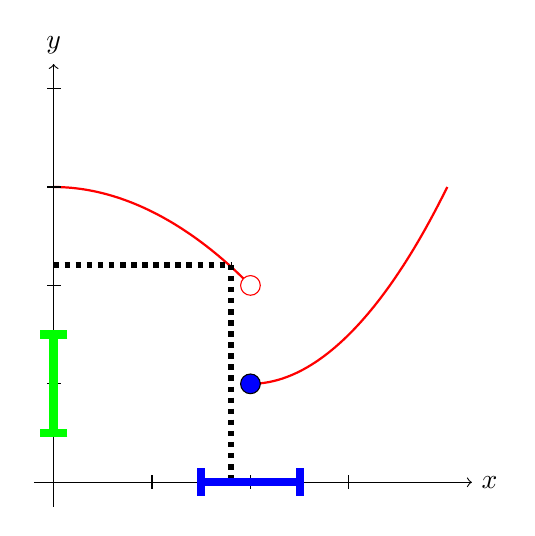
\begin{tikzpicture}[scale=1.25]
    \draw[red,thick] (0,3) parabola bend (0,3) (2,2.0);
    \draw[red,thick] (2,1.0) parabola bend (2,1.0) (4, 3.0); 
    \draw[red, fill=white] (2,2.0) circle (.1cm); 
    \draw[fill=blue] (2,1.0) circle (.1cm); 
    %\draw[loosely dotted] (0,0) grid (4,4);
    %\path[use as bounding box] (-2,-1) rectangle (5,5);
    \draw[->] (-0.2,0) -- (4.25,0) node[right] {$x$};
    \draw[->] (0,-0.25) -- (0,4.25) node[above] {$y$};
    \foreach \x/\xtext in {1/1, 2/2, 3/3}
    \draw[shift={(\x,0)}] (0pt,2pt) -- (0pt,-2pt) node[below] {};
    \foreach \y/\ytext in {1/1, 2/2, 3/3, 4/4}
    \draw[shift={(0,\y)}] (2pt,0pt) -- (-2pt,0pt) node[left] {};
    %\draw[dotted,line width=2pt] (0,1) -- (2,1);
    %\draw[dotted,line width=2pt] (2,1) -- (2,0);
    \draw[dotted,line width=2pt] (0,2.21) -- (1.8,2.21);
    \draw[dotted,line width=2pt] (1.8,2.21) -- (1.8,0);
    %\draw[green,line width=3pt] (0,0.5) -- (0,2.5);
    %\draw[green,line width=3pt] (4pt,0.5) -- (-4pt,0.5);
    %\draw[green,line width=3pt] (4pt,2.5) -- (-4pt,2.5);
   \draw[green,line width=3pt] (0,0.5) -- (0,1.5);
    \draw[green,line width=3pt] (4pt,0.5) -- (-4pt,0.5);
    \draw[green,line width=3pt] (4pt,1.5) -- (-4pt,1.5);

%    \draw[blue,line width=3pt] (0.5,0) -- (3.5,0);
 %  \draw[blue,line width=3pt] (0.5,4pt) -- (0.5,-4pt);
  %  \draw[blue,line width=3pt] (3.5,4pt) -- (3.5,-4pt);
 %     \draw[blue,line width=3pt] (1.0,0) -- (3.0,0);
  %  \draw[blue,line width=3pt] (1.0,4pt) -- (1.0,-4pt);
  %  \draw[blue,line width=3pt] (3.0,4pt) -- (3.0,-4pt);  
      \draw[blue,line width=3pt] (1.5,0) -- (2.5,0);
    \draw[blue,line width=3pt] (1.5,4pt) -- (1.5,-4pt);
    \draw[blue,line width=3pt] (2.5,4pt) -- (2.5,-4pt);  
%
    \end{tikzpicture}
\end{center}
\end{frame}


\addtocounter{framenumber}{-1}
\begin{frame}[fragile]{Computable functions are continuous}

\begin{center}

    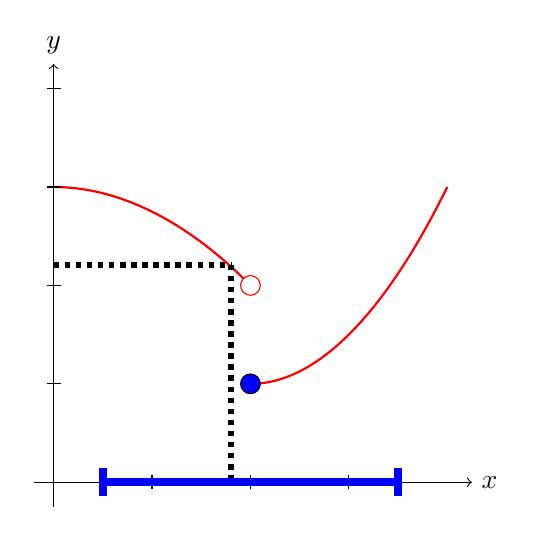
\begin{tikzpicture}[scale=1.25]
    \draw[red,thick] (0,3) parabola bend (0,3) (2,2.0);
    \draw[red,thick] (2,1.0) parabola bend (2,1.0) (4, 3.0); 
    \draw[red, fill=white] (2,2.0) circle (.1cm); 
    \draw[fill=blue] (2,1.0) circle (.1cm); 
    %\draw[loosely dotted] (0,0) grid (4,4);
    %\path[use as bounding box] (-2,-1) rectangle (5,5);
    \draw[->] (-0.2,0) -- (4.25,0) node[right] {$x$};
    \draw[->] (0,-0.25) -- (0,4.25) node[above] {$y$};
    \foreach \x/\xtext in {1/1, 2/2, 3/3}
    \draw[shift={(\x,0)}] (0pt,2pt) -- (0pt,-2pt) node[below] {};
    \foreach \y/\ytext in {1/1, 2/2, 3/3, 4/4}
    \draw[shift={(0,\y)}] (2pt,0pt) -- (-2pt,0pt) node[left] {};
    %\draw[dotted,line width=2pt] (0,1) -- (2,1);
    %\draw[dotted,line width=2pt] (2,1) -- (2,0);
    \draw[dotted,line width=2pt] (0,2.21) -- (1.8,2.21);
    \draw[dotted,line width=2pt] (1.8,2.21) -- (1.8,0);
    %\draw[green,line width=3pt] (0,0.5) -- (0,2.5);
    %\draw[green,line width=3pt] (4pt,0.5) -- (-4pt,0.5);
    %\draw[green,line width=3pt] (4pt,2.5) -- (-4pt,2.5);
    %\draw[green,line width=3pt] (0,0.5) -- (0,1.5);
    %\draw[green,line width=3pt] (4pt,0.5) -- (-4pt,0.5);
    %\draw[green,line width=3pt] (4pt,1.5) -- (-4pt,1.5);

    \draw[blue,line width=3pt] (0.5,0) -- (3.5,0);
   \draw[blue,line width=3pt] (0.5,4pt) -- (0.5,-4pt);
    \draw[blue,line width=3pt] (3.5,4pt) -- (3.5,-4pt);
 %     \draw[blue,line width=3pt] (1.0,0) -- (3.0,0);
   % \draw[blue,line width=3pt] (1.0,4pt) -- (1.0,-4pt);
   % \draw[blue,line width=3pt] (3.0,4pt) -- (3.0,-4pt);  
   %   \draw[blue,line width=3pt] (1.5,0) -- (2.5,0);
   % \draw[blue,line width=3pt] (1.5,4pt) -- (1.5,-4pt);
   % \draw[blue,line width=3pt] (2.5,4pt) -- (2.5,-4pt);  
%
    \end{tikzpicture}
\end{center}
\end{frame}


\addtocounter{framenumber}{-1}
\begin{frame}[fragile]{Computable functions are continuous}

\begin{center}

    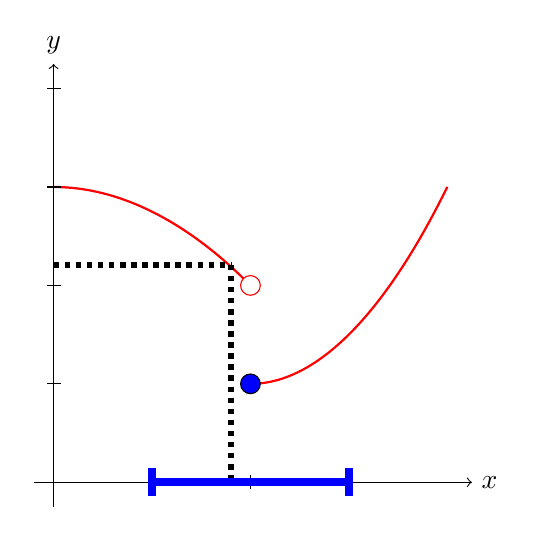
\begin{tikzpicture}[scale=1.25]
    \draw[red,thick] (0,3) parabola bend (0,3) (2,2.0);
    \draw[red,thick] (2,1.0) parabola bend (2,1.0) (4, 3.0); 
    \draw[red, fill=white] (2,2.0) circle (.1cm); 
    \draw[fill=blue] (2,1.0) circle (.1cm); 
    %\draw[loosely dotted] (0,0) grid (4,4);
    %\path[use as bounding box] (-2,-1) rectangle (5,5);
    \draw[->] (-0.2,0) -- (4.25,0) node[right] {$x$};
    \draw[->] (0,-0.25) -- (0,4.25) node[above] {$y$};
    \foreach \x/\xtext in {1/1, 2/2, 3/3}
    \draw[shift={(\x,0)}] (0pt,2pt) -- (0pt,-2pt) node[below] {};
    \foreach \y/\ytext in {1/1, 2/2, 3/3, 4/4}
    \draw[shift={(0,\y)}] (2pt,0pt) -- (-2pt,0pt) node[left] {};
    %\draw[dotted,line width=2pt] (0,1) -- (2,1);
    %\draw[dotted,line width=2pt] (2,1) -- (2,0);
    \draw[dotted,line width=2pt] (0,2.21) -- (1.8,2.21);
    \draw[dotted,line width=2pt] (1.8,2.21) -- (1.8,0);
    %\draw[green,line width=3pt] (0,0.5) -- (0,2.5);
    %\draw[green,line width=3pt] (4pt,0.5) -- (-4pt,0.5);
    %\draw[green,line width=3pt] (4pt,2.5) -- (-4pt,2.5);
    %\draw[green,line width=3pt] (0,0.5) -- (0,1.5);
    %\draw[green,line width=3pt] (4pt,0.5) -- (-4pt,0.5);
    %\draw[green,line width=3pt] (4pt,1.5) -- (-4pt,1.5);

%    \draw[blue,line width=3pt] (0.5,0) -- (3.5,0);
 %  \draw[blue,line width=3pt] (0.5,4pt) -- (0.5,-4pt);
  %  \draw[blue,line width=3pt] (3.5,4pt) -- (3.5,-4pt);
      \draw[blue,line width=3pt] (1.0,0) -- (3.0,0);
    \draw[blue,line width=3pt] (1.0,4pt) -- (1.0,-4pt);
    \draw[blue,line width=3pt] (3.0,4pt) -- (3.0,-4pt);  
   %   \draw[blue,line width=3pt] (1.5,0) -- (2.5,0);
   % \draw[blue,line width=3pt] (1.5,4pt) -- (1.5,-4pt);
   % \draw[blue,line width=3pt] (2.5,4pt) -- (2.5,-4pt);  
%
    \end{tikzpicture}
\end{center}
\end{frame}

\addtocounter{framenumber}{-1}
\begin{frame}[fragile]{Computable functions are continuous}

\begin{center}

    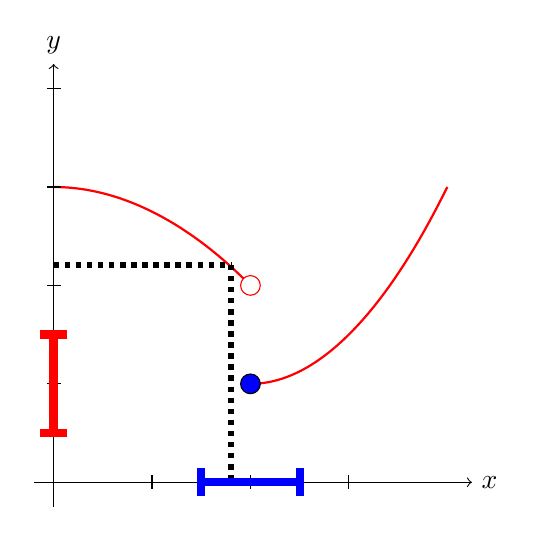
\begin{tikzpicture}[scale=1.25]
    \draw[red,thick] (0,3) parabola bend (0,3) (2,2.0);
    \draw[red,thick] (2,1.0) parabola bend (2,1.0) (4, 3.0); 
    \draw[red, fill=white] (2,2.0) circle (.1cm); 
    \draw[fill=blue] (2,1.0) circle (.1cm); 
    %\draw[loosely dotted] (0,0) grid (4,4);
    %\path[use as bounding box] (-2,-1) rectangle (5,5);
    \draw[->] (-0.2,0) -- (4.25,0) node[right] {$x$};
    \draw[->] (0,-0.25) -- (0,4.25) node[above] {$y$};
    \foreach \x/\xtext in {1/1, 2/2, 3/3}
    \draw[shift={(\x,0)}] (0pt,2pt) -- (0pt,-2pt) node[below] {};
    \foreach \y/\ytext in {1/1, 2/2, 3/3, 4/4}
    \draw[shift={(0,\y)}] (2pt,0pt) -- (-2pt,0pt) node[left] {};
    %\draw[dotted,line width=2pt] (0,1) -- (2,1);
    %\draw[dotted,line width=2pt] (2,1) -- (2,0);
    \draw[dotted,line width=2pt] (0,2.21) -- (1.8,2.21);
    \draw[dotted,line width=2pt] (1.8,2.21) -- (1.8,0);
    %\draw[green,line width=3pt] (0,0.5) -- (0,2.5);
    %\draw[green,line width=3pt] (4pt,0.5) -- (-4pt,0.5);
    %\draw[green,line width=3pt] (4pt,2.5) -- (-4pt,2.5);
    \draw[red,line width=3pt] (0,0.5) -- (0,1.5);
    \draw[red,line width=3pt] (4pt,0.5) -- (-4pt,0.5);
    \draw[red,line width=3pt] (4pt,1.5) -- (-4pt,1.5);

%    \draw[blue,line width=3pt] (0.5,0) -- (3.5,0);
 %  \draw[blue,line width=3pt] (0.5,4pt) -- (0.5,-4pt);
  %  \draw[blue,line width=3pt] (3.5,4pt) -- (3.5,-4pt);
 %     \draw[blue,line width=3pt] (1.0,0) -- (3.0,0);
  %  \draw[blue,line width=3pt] (1.0,4pt) -- (1.0,-4pt);
  %  \draw[blue,line width=3pt] (3.0,4pt) -- (3.0,-4pt);  
      \draw[blue,line width=3pt] (1.5,0) -- (2.5,0);
    \draw[blue,line width=3pt] (1.5,4pt) -- (1.5,-4pt);
    \draw[blue,line width=3pt] (2.5,4pt) -- (2.5,-4pt);  
%
    \end{tikzpicture}
\end{center}
\end{frame}

\addtocounter{framenumber}{-1}
\begin{frame}[fragile]{Computable functions are continuous}

\begin{center}

    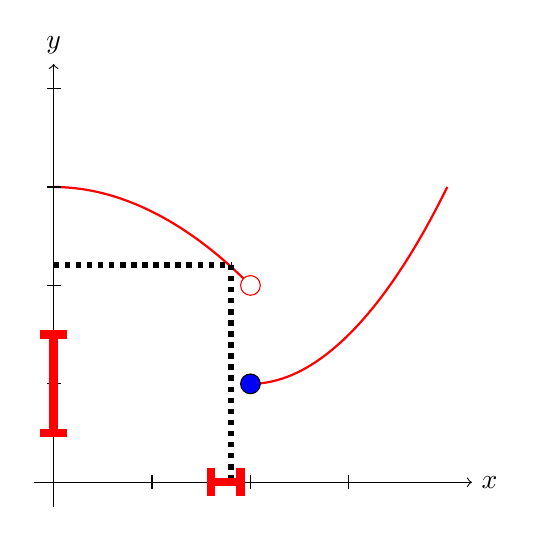
\begin{tikzpicture}[scale=1.25]
    \draw[red,thick] (0,3) parabola bend (0,3) (2,2.0);
    \draw[red,thick] (2,1.0) parabola bend (2,1.0) (4, 3.0); 
    \draw[red, fill=white] (2,2.0) circle (.1cm); 
    \draw[fill=blue] (2,1.0) circle (.1cm); 
    %\draw[loosely dotted] (0,0) grid (4,4);
    %\path[use as bounding box] (-2,-1) rectangle (5,5);
    \draw[->] (-0.2,0) -- (4.25,0) node[right] {$x$};
    \draw[->] (0,-0.25) -- (0,4.25) node[above] {$y$};
    \foreach \x/\xtext in {1/1, 2/2, 3/3}
    \draw[shift={(\x,0)}] (0pt,2pt) -- (0pt,-2pt) node[below] {};
    \foreach \y/\ytext in {1/1, 2/2, 3/3, 4/4}
    \draw[shift={(0,\y)}] (2pt,0pt) -- (-2pt,0pt) node[left] {};
    %\draw[dotted,line width=2pt] (0,1) -- (2,1);
    %\draw[dotted,line width=2pt] (2,1) -- (2,0);
    \draw[dotted,line width=2pt] (0,2.21) -- (1.8,2.21);
    \draw[dotted,line width=2pt] (1.8,2.21) -- (1.8,0);
    %\draw[green,line width=3pt] (0,0.5) -- (0,2.5);
    %\draw[green,line width=3pt] (4pt,0.5) -- (-4pt,0.5);
    %\draw[green,line width=3pt] (4pt,2.5) -- (-4pt,2.5);
    \draw[red,line width=3pt] (0,0.5) -- (0,1.5);
    \draw[red,line width=3pt] (4pt,0.5) -- (-4pt,0.5);
    \draw[red,line width=3pt] (4pt,1.5) -- (-4pt,1.5);

%    \draw[blue,line width=3pt] (0.5,0) -- (3.5,0);
 %  \draw[blue,line width=3pt] (0.5,4pt) -- (0.5,-4pt);
  %  \draw[blue,line width=3pt] (3.5,4pt) -- (3.5,-4pt);
 %     \draw[blue,line width=3pt] (1.0,0) -- (3.0,0);
  %  \draw[blue,line width=3pt] (1.0,4pt) -- (1.0,-4pt);
  %  \draw[blue,line width=3pt] (3.0,4pt) -- (3.0,-4pt);  
      \draw[red,line width=3pt] (1.6,0) -- (1.9,0);
    \draw[red,line width=3pt] (1.6,4pt) -- (1.6,-4pt);
    \draw[red,line width=3pt] (1.9,4pt) -- (1.9,-4pt);  
%
    \end{tikzpicture}
\end{center}
\end{frame}


